\section{Iterated Sparse Approximation Framework}

\begin{figure}[h]
\centering
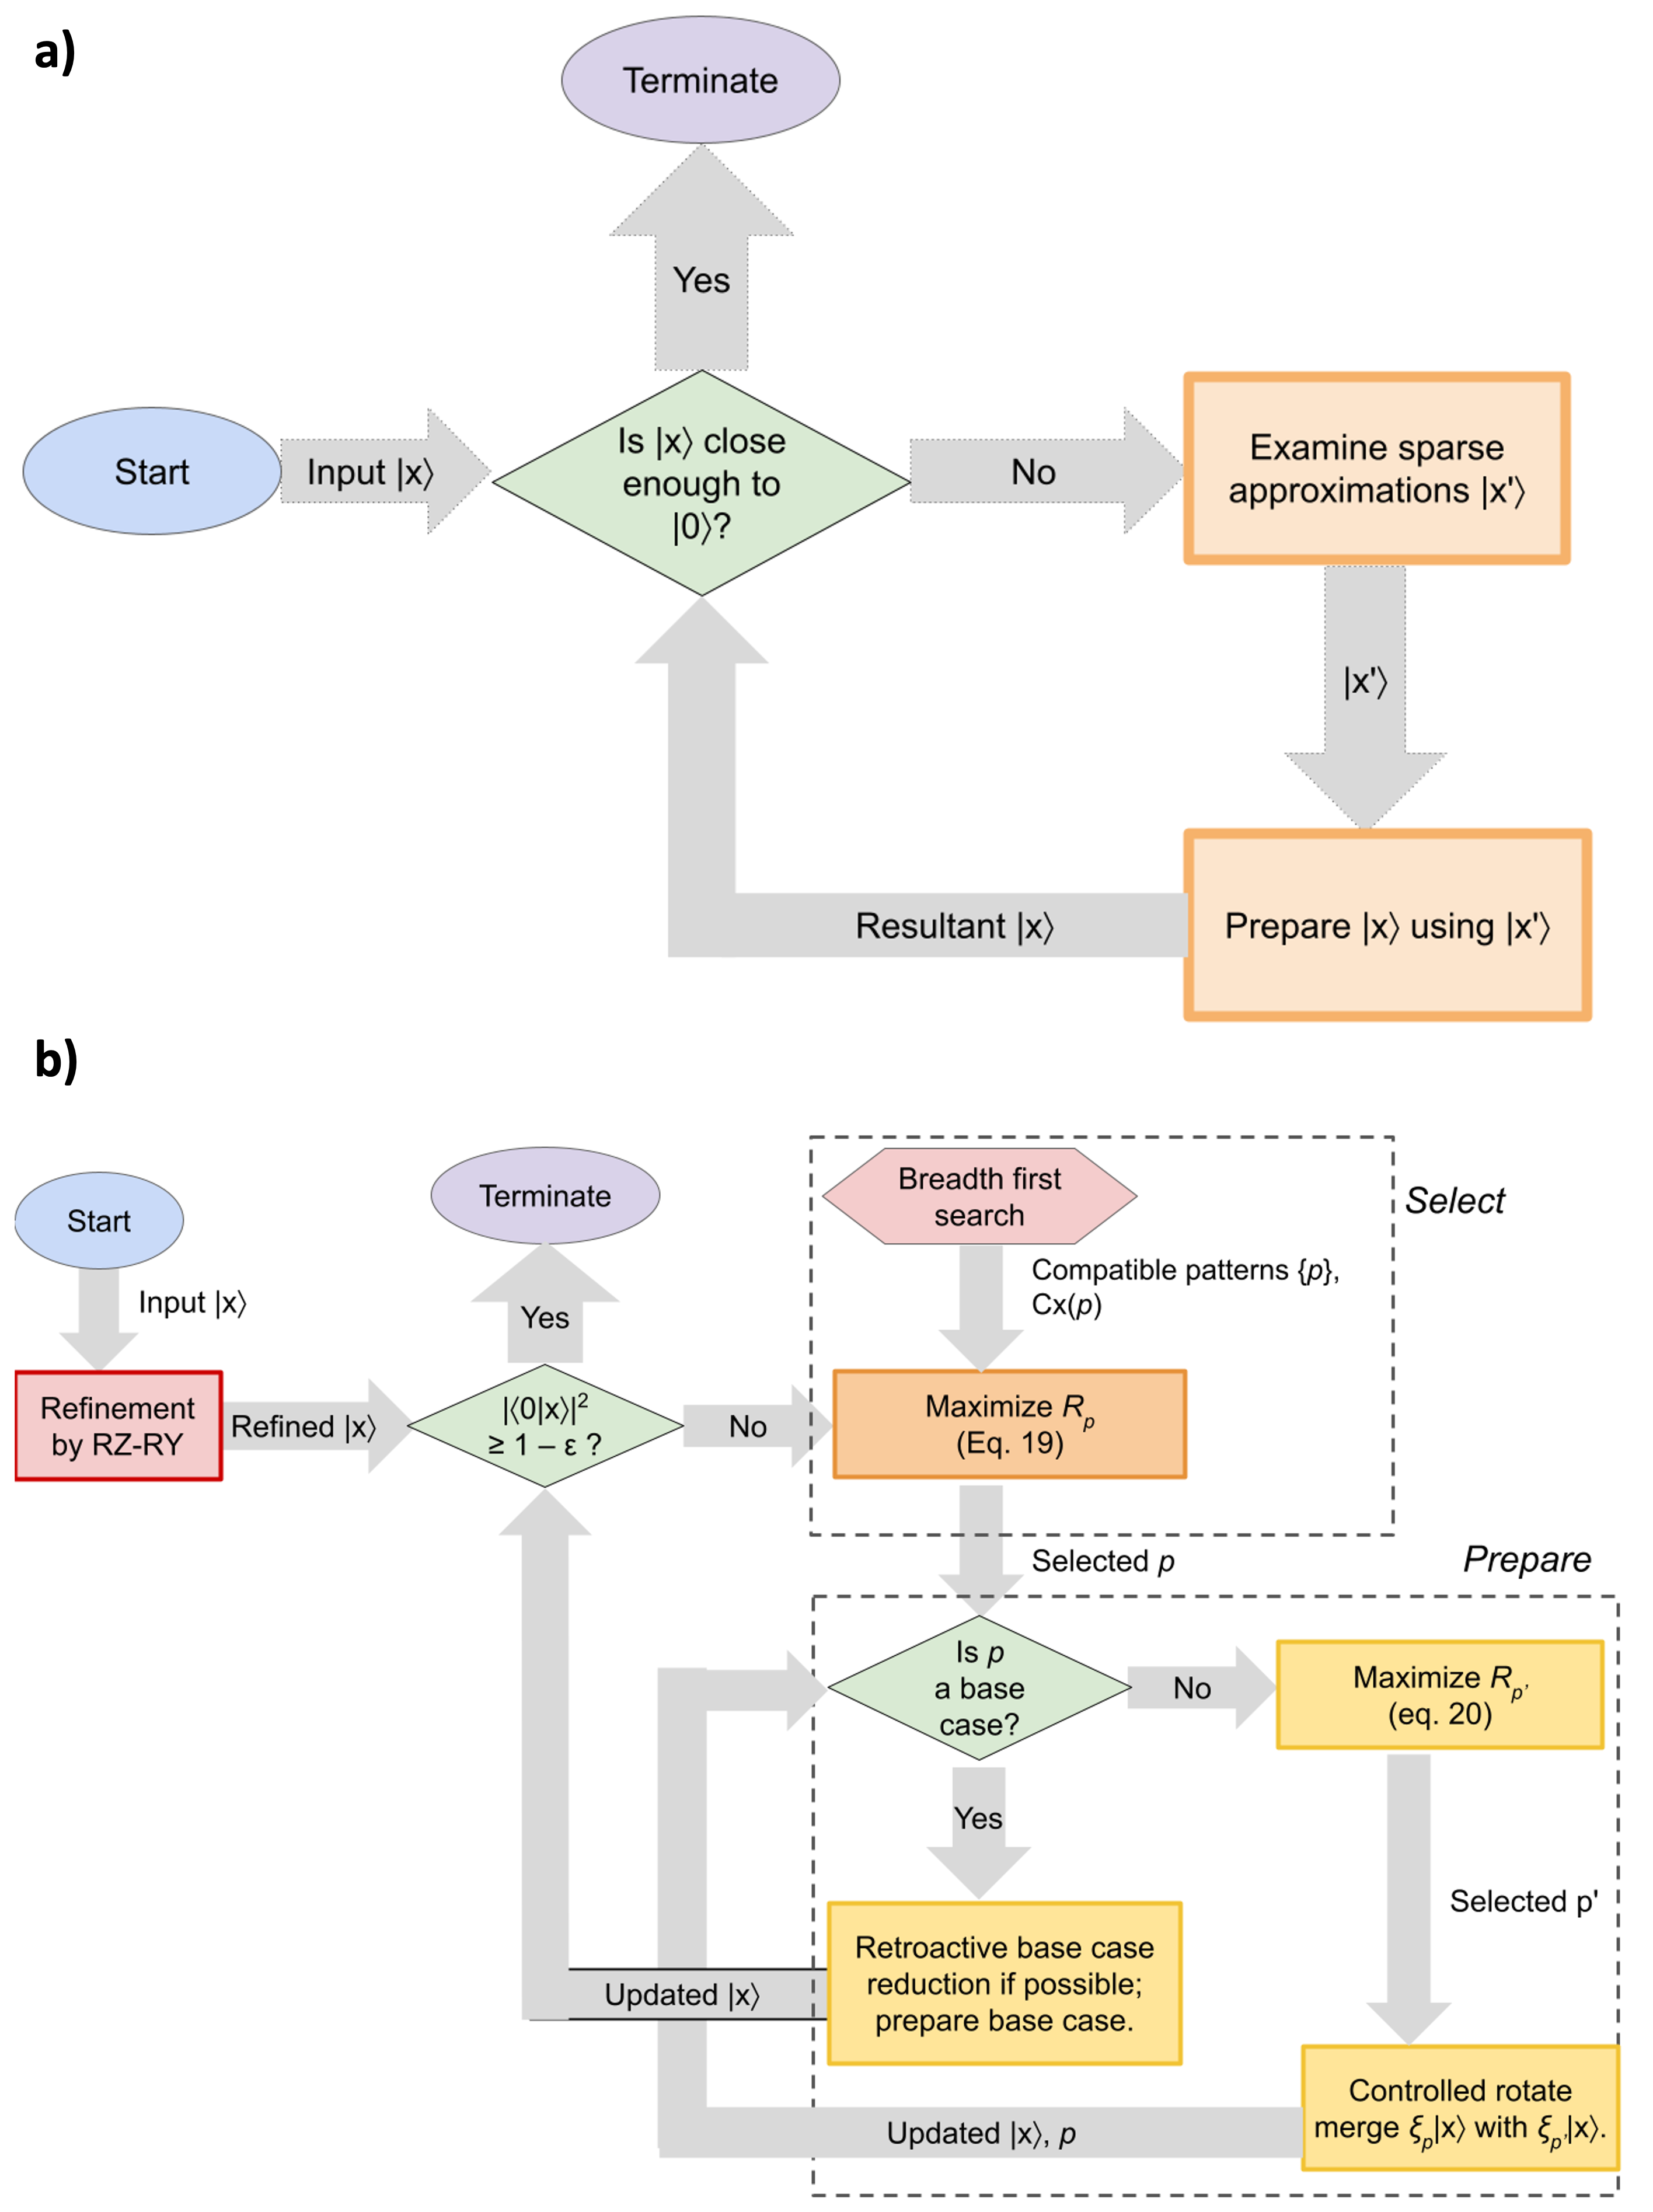
\includegraphics[width=0.8\linewidth]{main/figs/mfig_1.png}
\caption{Schematic depiction of the ISA framework. a) The ISA framework is a
check termination-select-prepare loop that brings $\ket{x}$ closer to $\ket{\mathbf{0}}$
on every iteration. b)  Flowchart depiction of the ISA implementation which includes Refinement by RZ-RY before entering the
main check termination-select-prepare loop}
\label{mfig1}
\end{figure}

\subsection{Quantum state preparation}
QSP is formally defined as: given an arbitrary quantum state $\ket{x}$ and a
family of quantum gates $G$, return a sequence of quantum gates 
$h_1, h_2, ... , h_m$ from $G$ such that $h_m ... h_2h_1\ket{\mathbf{0}} = \ket{x}$
\cite{1629135}. In this paper, we assume $G$ contains continuously parameterized 
RX, RY, and RZ gates, as well as the CX gate. This gate set is chosen because 
these gates are both easy to reason about and easy to compile into the native 
gate set of existing quantum computers \cite{maldonado2022error}. 

\begin{equation}
\label{eq1}
g_m ... g_2g_1\ket{x} = \ket{y}
\end{equation}
\begin{equation}
\label{eq2}
|\braket{y|\mathbf{0}}|^2 \geq 1 - \epsilon
\end{equation}
\begin{align}
\label{eq3}
|\braket{x|x'}|^2 &= |\braket{x|g_1^\dagger g_2^\dagger ... g_m^\dagger|\mathbf{0}}|^2 
\nonumber\\
&= |\braket{y|\mathbf{0}}|^2 \geq 1 - \epsilon.
\end{align}
In this work, we tackle the following version of approximate QSP: given an
arbitrary quantum state $\ket{x}$, return a sequence of quantum gates 
$g_1, g_2, ..., g_m$ that satisfies Eq. 1.  Eq. 2 represents the state preparation fidelity requirement with $\epsilon$ as the fidelity error.

This version of approximate QSP can be applied towards approximately preparing
arbitrary quantum states. For some state $\ket{x}$, if a sequence of gates can
be found for transforming $\ket{x}$ to $\ket{y}$, such that $\ket{y}$ is close
to $\ket{\mathbf{0}}$, then inverting each gate and reversing the gate sequence generates
a gate sequence for approximately preparing $\ket{x}$ starting from $\ket{\mathbf{0}}$.
Indeed, if $\ket{y} = g_m ... g_2g_1\ket{x}$, 
$|\braket{\mathbf{0}|y}|^2 \geq 1 - \epsilon$, and 
$\ket{x'} = g_1^\dagger g_2^\dagger ... g_m^\dagger\ket{\mathbf{0}}$, then Eq. 3 follows. This indicates that the prepared state $\ket{x'}$ is a good approximation of the
target state $\ket{x}$. For this work, qubit indices start at zero and start from the right. This means
$\ket{0010}$ is the result of applying an $X$ gate to qubit 1 of $\ket{0000}$.
Single-qubit rotations are written with the rotation angle first, then the qubit
index. For example, an RZ gate, angle $\frac{\pi}{2}$, applied to qubit 1, is
written as RZ$(\frac{\pi}{2}, 1)$. CX gates are written with the control qubit 
first. For example, a CX gate applied to qubit 2, with qubit 1 as the control,
is written as CX$(1, 2)$. Unless otherwise specified, $n$ will represent the
number of qubits in the system and $N = 2^n$ will represent the number of
amplitudes to be encoded onto those $n$ qubits. In addition, 
$\ket{0}^{\otimes n}$, the starting state of an $n$-qubit quantum processor, 
will be abbreviated as $\ket{\mathbf{0}}$.

\subsection{Patterns and Substates}
A $k$-bit pattern denoted by $p$ over $n$-qubits is defined as a length-$n$ string 
$\{0, 1, *\}^n$ containing exactly $k$ `$*$' characters. The parameter $k$
may be zero, in which case $p$ would be a length-$n$ bit-string. Let $I_p$ denote the set of $2^k$ integers such that, integer $i\in I_p$ is a permutation of the $k$-bit pattern formed by replacing $*$ with 0 or 1. Next, define the $p$-substate of a quantum state $\ket{x}$ with the operator $\xi_p$ as shown in Eq. 5.
\begin{equation}
    \label{eq5}
     \xi_p\ket{x} = \sum_{i \in I_p}{\ket{i}\braket{i|x}} 
\end{equation}
When $\ket{x}$ is written in the computational basis, $\xi_p\ket{x}$ contains the 
subset of basis states $\ket{i}$ where $i$ matches $p$. In most cases, the norm of $\xi_p\ket{x}$ is less than 1, and therefore does not represent a proper quantum state, 
but is instead a complex-valued vector. Still, we define the action of quantum gates
on these substates as we would for normalized quantum states. Substates are defined analogously for quantum state-derived functionals as $(\xi_p\ket{x})^\dagger = \bra{x}\xi_p$.

An X or CX gate may be applied to a pattern $p$ as long as their relevant qubit
indices do not correspond to indices where $p$ has a `$*$'.
If an X gate targeting
qubit $i$ is applied to a pattern $p$, the result is $p$ but with the $i$'th
character inverted from 0 to 1 or vice versa. If a CX gate with control qubit $i$
and target qubit $j$ is applied to $p$ and $p_i = 0$, the result is $p$; otherwise,
the result is $p$ but with the $j$'th character inverted. This behavior of X and CX
gates on patterns is chosen to match the behavior of those gates on substates, 
as described in Lemma 1 in the Supplementary Information; because of this relationship, we let $g(p)$ denote the
result of applying a gate $g$ to a pattern $p$.

\subsection{Substate Merging}\label{substate_merge}
Our implementation of the ISA framework makes extensive use of a substate merging
subroutine, which we describe here. Given a quantum state $\ket{x}$, a $k$-bit
pattern $p$, and an $X$ gate $g$ that can be applied to $p$ that follows $g(p) \neq p$, the 
substate merging subroutine applies a single qubit rotation $R$ to $\ket{x}$ such
that the norm of $\xi_pR\ket{x}$ is maximized. Any single qubit rotation can be decomposed into an RZ-RY-RZ sequence. Since RZ
gates only apply complex phases to the amplitudes in the computational basis, the
last RZ has no effect on the norm of $\xi_pR\ket{x}$ and can be left out. Thus, we
parameterize $R = RY(\theta)RZ(\phi)$. To compute the optimal $\theta$ and $\phi$, we perform casework on $p[i]$. If
$p[i] = 0$, then $g(p)[i] = 1$, while the norm objective function can be denoted by:
\begin{align}
\label{eq7}
\xi_pR\ket{x} &= \xi_pRY(\theta)RZ(\phi)\ket{x} \nonumber \\
 &= cos(\frac{\theta}{2})\xi_p\ket{x} - e^{i\phi}sin(\frac{\theta}{2})\xi_pg\ket{x} \quad \textit{(ignoring global phase)}.
\end{align}
The squared norm of this vector is then:
% \begin{align}
% % |\xi_pR\ket{x}|^2 &= \left(cos(\frac{\theta}{2})\bra{x}_p 
% %   - e^{-i\phi}sin(\frac{\theta}{2})(\bra{x}g)_p\right)
% %   \left(cos(\frac{\theta}{2})\ket{x}_p 
% %   - e^{i\phi}sin(\frac{\theta}{2})(g\ket{x})_p\right) \nonumber \\

% |\xi_pR\ket{x}|^2 &= cos^2(\frac{\theta}{2})\bra{x}\xi_p\ket{x} 
%   - 2cos(\frac{\theta}{2})sin(\frac{\theta}{2})\text{Re}(e^{-i\phi}
%   \bra{x}g^\dagger\xi_p\ket{x} \nonumber \\
%   & + sin^2(\frac{\theta}{2})\bra{x}_p g^\dagger \xi_p g\ket{x} \nonumber \\

%     &= cos^2(\frac{\theta}{2})\bra{x}\xi_p\ket{x} 
%   - 2cos(\frac{\theta}{2})sin(\frac{\theta}{2})\text{Re}
%   (e^{-i\phi}\bra{x}\xi_{gp}g\xi_p\ket{x}) \nonumber \\
%   &\quad + sin^2(\frac{\theta}{2})\bra{x}\xi_{gp}\ket{x},
  
% \end{align}

\begin{align}
\label{eq8}
    |\xi_pR\ket{x}|^2 &= cos^2(\frac{\theta}{2})\bra{x}\xi_p\ket{x} 
  - 2cos(\frac{\theta}{2})sin(\frac{\theta}{2})\text{Re}(e^{-i\phi}
  \bra{x}g^\dagger\xi_p\ket{x} \nonumber \\
  & + sin^2(\frac{\theta}{2})\bra{x}_p g^\dagger \xi_p g\ket{x} \\
  &= cos^2(\frac{\theta}{2})\bra{x}\xi_p\ket{x} 
  - 2cos(\frac{\theta}{2})sin(\frac{\theta}{2})\text{Re}
  (e^{-i\phi}\bra{x}\xi_{g(p)}g\xi_p\ket{x}) \nonumber \\
  &\quad + sin^2(\frac{\theta}{2})\bra{x}\xi_{g(p)}\ket{x} \nonumber
\end{align}
where the last step used Lemma 1 to simplify. The first and third terms of
this expression are non-negative, and do not depend on the sign of $\theta$.
Therefore, $\theta$ can be chosen such that the coefficient
$2cos(\frac{\theta}{2})sin(\frac{\theta}{2})$ of the second term is negative.
Following this, the expression is maximized when $e^{-i\phi}\bra{x}\xi_{g(p)}g\xi_p\ket{x}$
is a positive real number with no imaginary part, which is achieved by assigning $\phi = \text{phase}(\bra{x} \xi_{g(p)} g \xi_p\ket{x}).$
Performing this substitution and simplifying using half-angle laws yields Eq. 9. This quantity is maximized when $\theta$ satisfies Eq. 10.
\begin{align}
\label{eq9}
% |(R\ket{x})_p|^2 &= cos^2(\frac{\theta}{2})\bra{x}_p\ket{x}_p 
%   - 2cos(\frac{\theta}{2})sin(\frac{\theta}{2})|\bra{x}_{gp}g\ket{x}_p| 
%   + sin^2(\frac{\theta}{2})\bra{x}_{gp}\ket{x}_{gp} \nonumber \\
% &= \frac{1}{2}(1 + cos(\theta))\bra{x}_p\ket{x}_p 
%   - sin(\theta)|\bra{x}_{gp}g\ket{x}_p| 
%   + \frac{1}{2}(1 - cos(\theta))\bra{x}_{gp}\ket{x}_{gp} \nonumber \\
% &= \frac{1}{2}(\bra{x}_p\ket{x}_p + \bra{x}_{gp}\ket{x}_{gp})
%    + \frac{1}{2}cos(\theta)(\bra{x}_p\ket{x}_p - \bra{x}_{gp}\ket{x}_{gp})
%    + sin(\theta)|\bra{x}_{gp}g\ket{x}_p\\
|(R\ket{x})_p|^2 &= \frac{\bra{x}\xi_p\ket{x} + \bra{x}\xi_{g(p)}\ket{x}}{2}  + \frac{cos(\theta)}{2} \{\bra{x}\xi_p\ket{x} - \bra{x}\xi_{g(p)}\ket{x}\} \\ \nonumber
& - sin(\theta)| \bra{x}\xi_{g(p)}\xi_p\ket{x} |
\end{align}

\begin{align}
\label{eq10}
% \theta &= -arccos\left(\frac{A}{\sqrt{A^2 + B^2}}\right) \nonumber \\
% A &= \frac{1}{2}(\bra{x}_p\ket{x}_p - \bra{x}_{gp}\ket{x}_{gp}) \nonumber \\
% B &= |\bra{x}_{gp}g\ket{x}_p| \\
\theta = tan^{-1} \frac{-2| \bra{x}\xi_{g(p)}\xi_p\ket{x} |}{\bra{x}\xi_p\ket{x} - \bra{x}\xi_{g(p)}\ket{x}} 
\end{align}


Alternatively, in the case of $p[i] = 1$ and $g(p)[i] = 0$, $ \xi_pR\ket{x} $ follows Eq. 11 ignoring global phase. Performing the same calculations as above, the magnitude of this state is maximized when conditions in Eq. 12 are satisfied. By determining $\theta$ and $\phi$, $R$ can be constructed. This procedure of determining $\theta$ and $\phi$ to maximize norm of $\xi_pR\ket{x}$ is called substate merging because Eq. 7 and 
Eq. 11 show that the final substate, $\xi_p R\ket{x}$, is a linear
combination of $\xi_p\ket{x}$ and $\xi_{g(p)}\ket{x}$. This can be considered analogous to merging $\xi_{g(p)}\ket{x}$ with $\xi_p\ket{x}$ to form a new, larger-magnitude substate
$\xi_p R\ket{x}$, while some residue is left behind at $\xi_{g(p)}R\ket{x}$. For this
reason, the substate merging procedure will be described as ``merging $\xi_{g(p)}\ket{x}$ into $\xi_p\ket{x}$.''

\begin{equation}\label{eq11}
\xi_p R\ket{x} = sin(\frac{\theta}{2})\xi_p g\ket{x} + e^{i\phi}cos(\frac{\theta}{2})\xi_p\ket{x}.
\end{equation}

\begin{align}
\label{eq12}
\theta &= tan^{-1} \frac{2| \bra{x}\xi_{g(p)}\xi_p\ket{x} |}{\bra{x}\xi_p\ket{x} - \bra{x}\xi_{g(p)}\ket{x}} \nonumber \\
\phi &= \text{phase}(\bra{x} \xi_{g(p)} g \xi_p\ket{x})
\end{align}



In most cases, the substate merging procedure needs to be modified such that it
doesn't disturb the amplitude at $\ket{\mathbf{0}}$. We call this modified procedure
``controlled substate merging" and define it as follows. Given a quantum state
$\ket{x}$, a pattern $p$, and a CX gate $g$ that can be applied to $p$ (and
$g(p) \neq p$), the
controlled substate merging procedure applies a transformation $R$ consisting
of the CX gate $g$ and single-qubit rotations applied to the target qubit of
$g$, such that the norm of $\xi_p R\ket{x} $ is maximized and
$\bra{\mathbf{0}}R\ket{x} = \braket{\mathbf{0}|x}$, ignoring global phase.

The substate merging procedure can be adapted for controlled substate merging 
as follows. First, the
RZ-RY sequence $R'$ is constructed for merging $\xi_p\ket{x}$ into $\xi_{g(p)}\ket{x}$ as shown in Eq. 13. In this pair of gates, only the RY gate disturbs
the amplitude at $\ket{0}$, thus, the RY gate is replaced with a controlled-RY
gate, then decomposed into CX and RY described in Eq. 14 wherein $g$ is the CX gate given in the problem statement. The transformation $R'$
minimizes $\xi_pR'\ket{x}$ and maximizes $\xi_{g(p)}R'\ket{x}$, whereas the opposite effect is desired. This problem is tackled by removing the trailing $g$ in the
gate sequence $R'$ to get the desired gate sequence $R$ in Eq. 15. One interesting property of this construction is that, for all
integers $i$ where $g\ket{i} = \ket{i}$, $\braket{i|R|x} = \braket{i|x}$ up to
a complex phase, and the restriction $\braket{\mathbf{0}|R|x} = \braket{\mathbf{0}|x}$ is a special
case of this more general property of the construction for controlled substate
merging. This property will prove useful for our ISA implementation.

\begin{equation} \label{eq13}
R' = RY(\theta)RZ(\phi).
\end{equation}
\begin{align} \label{eq14}
R' &= CRY(\theta)RZ(\phi) \nonumber \\
&= gRY(-\frac{\theta}{2})gRY(\frac{\theta}{2})RZ(\phi)
\end{align}

\begin{equation} \label{eq15}
R = RY(\frac{\theta}{2})gRY(\frac{\theta}{2})RZ(\phi).
\end{equation}

\subsection{Sparse quantum state preparation}
In this work, we consider sparse quantum states of the form:
\begin{equation}
\ket{x'} = \sum_{i \in I_{p^0}}{c_i\ket{i}} + \sum_{j \in I_p}{c_j\ket{j}}
\end{equation}
where $p$ is a $k$-bit pattern, $k \leq 2$, $p^0$ is $p$ but with its `1'
characters changed to `0', and $p \neq p^0$. We also require the `$*$' 
characters in $p$ to be adjacent to each other, if there are two of them, and 
for all pairs $k$ and $l$ where $p[k] = p[l] = 1$, there exists no $m$ such 
that $k < m < l$ and $p[m] = $ `$*$'. Patterns meeting these latter two criteria 
regarding the positioning of `1' and `$*$' characters are called ``compatible'',
since these criteria are necessary for our sparse QSP method to work on LNN 
architectures specifically. For example, `$011**0$', `$100*$', and `$00001$' are
compatible patterns, but `$01*001$' and `$00*01*$' are not.

As a base case, if $p$ contains at most one `1' character, and that character 
is adjacent to a `$*$' character, then $\ket{x'}$ is a $k + 1$-qubit entangled state on neighboring qubits. In addition, $k + 1 \leq 3$, so existing exact 
state preparation methods can be applied \cite{PhysRevA.77.032320}; 
we describe our specific implementation in the Appendix. Otherwise, we can
construct a sequence of CX gates $g_1, g_2, ..., g_m$ and a sequence of
patterns $p_0, p_1, ..., p_m$ such that $p_k = g_k(p_{k - 1})$ for all 
$1 \leq k \leq m$, $p_0 = p$, and $p_m$ is a base case pattern. This
construction is possible because $p$ satisfies the compatibility criteria
described above. From here, we construct the sequence 
$\ket{x'_0}, \ket{x'_1}, ..., \ket{x'_m}$ such that $\ket{x'_k} = g_k\ket{x'_{k-1}}$
and $\ket{x'_0} = \ket{x'}$.
Repeatedly applying Lemma 1 shows that
\begin{equation}
\ket{x'_m} = \sum_{i \in {I_{p^0}}}{c_i'\ket{i}} 
+ \sum_{j \in I_{p_m}}{c'_j\ket{j}}
\end{equation}
for some complex amplitudes $c'_i$ and $c'_j$. Then $\ket{x'_m}$ is a 
$k + 1$-qubit quantum state on neighboring qubits, which can be prepared by
existing methods. In summary, our sparse quantum state preparation method uses a
sequence of CX gates to move the $p$-substate to qubits adjancent to the 
$p^0$-substate, then applies exact QSP. The number of CX gates our method needs to prepare sparse quantum states is the 
minimum possible length $m$ of the CX gate sequence used to move the $p$-substate
plus the number of CX gates needed for the base case. Let $CX(p)$ denote this
quantity. Breadth-first search can be used to compute $CX(p)$; despite the
inefficiency of such an approach, the computation for $CX(p)$ can be 
precomputed
and cached, and therefore, needs to be performed only once.



\subsection{ISA Framework Implementation}
In the previous sections, we described the building blocks for our ISA
implementation; in this section, we assembled the pieces. For the select step, we enumerate all compatible $k$-bit patterns $p$, with 
$k \leq 2$. For each pattern, we construct the corresponding (non-normalized) sparse
approximation:
\begin{equation}
\ket{x'(p)} = \xi_{p^0}\ket{x} + \xi_p\ket{x}.
\end{equation}
When the sparse QSP method is applied to $\ket{x'(p)}$, the result is 
$\|x'(p)\| \ket{\mathbf{0}}$; when the same gate sequence is applied to $\ket{x}$ to get
$\ket{x_1}$, we expect $\braket{\mathbf{0}|x_1} = \|x'(p)\|$. This corresponds to a
fidelity increase of $\braket{x'(p)|x'(p)} - |\braket{\mathbf{0}|x}|^2$ using $CX(p$) CX gates, or a fidelity increase ratio of
\begin{equation}
R_p = \frac{\braket{x'(p)|x'(p)} - |\braket{\mathbf{0}|x}|^2}{1 + CX(p)}.
\end{equation}
Adding 1 to the denominator is necessary to prevent division by zero when $CX(p)$
is zero. In the select step, we greedily choose $p$ to maximize $R_p$ and select
the corresponding sparse approximation $\ket{x'(p)}$. In the prepare step, the sparse QSP method is adapted for general QSP. In our 
implementation, we replace the iterated application of CX gates to move the
$p$-substate with the iterated application of controlled substate merging. This
change allows the $p$-substate of $\ket{x}$ to increase its norm as it moves towards
a base-case pattern, instead of keeping the same norm throughout. Also, using
controlled substate merging in place of CX gates will not affect the $p^0$ substate,
as argued at the end of section \ref{substate_merge}. In addition, we implement a
greedy selection procedure to construct the pattern sequence $p_0, p_1, ..., p_m$.
Specifically, we implement prepare using the following procedure:
\begin{enumerate}
  \item If $p$ is a base case pattern, apply exact QSP and terminate the 
    prepare step.
  \item Otherwise, construct $\mathcal{P}$, the set of patterns $p'$ such that $g(p) = p'$ for
    some CX gate $g$ and $p \neq p'$.
  \item For each $p' \in \mathcal{P}$, compute the magnitude of the substate that would result
    from merging $\ket{x_p}$ with \xi_{p'}$\ket{x}$ and call this quantity $mag(p')$.
  \item For each $p'$, compute the projected fidelity increase ratio as
    \begin{equation}
      R_{p'} = \frac{mag(p') + \bra{x}\xi_{p^0}\ket{x} - |\braket{\mathbf{0}|x}|^2}
      {1 + \min(CX(p), CX(p'))}
    \end{equation}
    The numerator is the projected fidelity increase after substate merging, while
    the denominator is the projected number of CX gates - one for substate merging
    and $\min(CX(p), CX(p'))$ for preparing the resulting sparse approximation.
  \item Select $p'$ such that it maximizes $R_{p'}$. If 
    $CX(p) < CX(p')$, then controlled substate merge
    $\xi_{p'}\ket{x}$ into $\xi_{p}\ket{x}$ and return to the first step. 
    Otherwise, controlled substate merge $\xi_p\ket{x}$ into $\xi_{p'}\ket{x}$, set 
    $p = p'$, and return to the first step.
\end{enumerate}
It may seem possible that this procedure will always select $p'$ with
$CX(p') > CX(p)$ in step 5 and enter an infinite loop. However,
this cannot happen because each time another substate is merged into $\xi_p\ket{x}$, an
extra CX gate is used. This extra CX gate must be justified by a corresponding
increase in projected fidelity increase, and the projected fidelity increase cannot
increase indefinitely.



